\documentclass[runningheads,a4paper]{llncs}

\usepackage{amssymb}
\setcounter{tocdepth}{3}
\usepackage{graphicx}

%%%%%%%%%ADDED PACKAGES%%%%%%%%%%
\usepackage{amsmath}
\usepackage{graphicx}
\usepackage{booktabs}
\usepackage[caption=false]{subfig}
%%%%%%%%%%%%%%%%%%%%%%%%%%%%%%%%%

\usepackage{url}
\urldef{\mailsa}\path||
\urldef{\mailsb}\path||
\urldef{\mailsc}\path|simon.andermatt@unibas.ch|    
\newcommand{\keywords}[1]{\par\addvspace\baselineskip
\noindent\keywordname\enspace\ignorespaces#1}


\DeclareMathOperator*{\argmax}{arg\,max}
\begin{document}

\mainmatter  % start of an individual contribution

% first the title is needed
\title{Multi-Dimensional Gated Recurrent Units\\
for the Segmentation of Biomedical 3D-Data}

% a short form should be given in case it is too long for the running head
\titlerunning{Multi-Dimensional GRU for the Segmentation of Biomedical Data}

% the name(s) of the author(s) follow(s) next
%
% NB: Chinese authors should write their first names(s) in front of
% their surnames. This ensures that the names appear correctly in
% the running heads and the author index.
%
\author{Simon Andermatt \and Simon Pezold \and Philippe Cattin}
% index{Andermatt, Simon}
% index{Pezold, Simon}
% index{Cattin, Philippe}
%
\authorrunning{Multi-Dimensional GRU for the Segmentation of Biomedical Data}

% the affiliations are given next; don't give your e-mail address
% unless you accept that it will be published
\institute{Department of Biomedical Engineering, 
University of Basel,
Switzerland
\mailsc\\
}

%
% NB: a more complex sample for affiliations and the mapping to the
% corresponding authors can be found in the file "llncs.dem"
% (search for the string "\mainmatter" where a contribution starts).
% "llncs.dem" accompanies the document class "llncs.cls".
%

\toctitle{Multi-Dimensional Gated Recurrent Units for the Segmentation of Volumetric Biomedical Data}
\tocauthor{Simon Andermatt}
\maketitle


\begin{abstract}
We present a supervised deep learning method to automatically segment 3D volumes of biomedical image data. The presented method takes advantage of a neural network with the main layers consisting of multi-dimensional gated recurrent units. We apply an on-the-fly data augmentation technique which allows for accurate estimations without the need for either a huge amount of training data or advanced data pre- or postprocessing. We show that our method performs amongst the leading techniques on a popular brain segmentation challenge dataset in terms of speed, accuracy and memory efficiency. We describe in detail advantages over a similar method which uses the well-established long~short-term~memory.

\keywords{deep learning, GRU, multi-dimensional RNN, segmentation}
\end{abstract}


\section{Introduction}
With the rapid advancements of imaging technologies, their ubiquitous availability and dropping prices, vast amounts of data are collected. This is particularly true for medical imaging. Accurate segmentation and delineation of e.g. pathologies in this medical data, however, pose real challenges as this is still mainly a manual process. In late phase drug studies with thousands of patients, multiple 3d datasets with different MR sequences are often collected per patient. If quantitative analysis of the immense amount of data is required, the time that has to be spent on the data by trained experts is enormous. A successful automated segmentation technique would decrease manual work to a minimum, cutting the costs and time spent on developing new treatments.

Automatic segmentation of biomedical volumetric data is, however, a challenging problem due to its high dimensionality, imaging noise, artifacts and other factors. Recent advances in the field of deep learning, especially the enabling effect of modern GPUs along with the advent of general purpose GPU computing, led to a revival of convolutional neural networks~\cite{krizhevsky_imagenet_2012}. These feed-forward networks show great promise, but need a large number of layers to solve a difficult task accurately. A recurrent neural network (RNN), in contrast, can become arbitrarily deep due to its additional temporal dimension. Each timestep computed in an RNN corresponds roughly to one layer in a feed-forward network, with the weights in one RNN being the same for each timestep. This property allows defining substantially more complexity very elegantly without the need for a huge number of layers or parameters.

The multi-dimensional Long Short-Term Memory (MD-LSTM) proposed by Stollenga et al.~\cite{stollenga_parallel_2015}, called \textit{PyraMiD-LSTM}, applied these insights to the Long Short-Term Memory (LSTM)~\cite{hochreiter1997long}. It defines two LSTMs for each spatial dimension, using said spatial dimension as temporal dimension. The first one processes the data along that dimension, the second one in the opposite direction. In order to make full use of the spatial information, not only the direct predecessor along the temporal direction is taken into account, but also its local neighborhood. This can be neatly expressed using convolutions. 

A relatively new RNN called Gated Recurrent Unit (GRU)~\cite{cho_learning_2014} grew popular in recent years and became a strong competitor for the LSTM. It can be seen as a simplified version of the LSTM, which uses an update gate instead of a forget and input gate and combines the hidden and cell state~\cite{olah_understanding_2015}. It has been shown that it performs comparably to the LSTM in the task of sequence modeling~\cite{chung_empirical_2014}. Another study suggests that GRU and LSTM report similar performance on selected tasks~\cite{greff_lstm:_2015}. An empirical search among more than 10\,000 RNN architectures showed that on the selected tasks, although not the best performing RNN on every task, the GRU outperformed the standard LSTM architecture~\cite{jozefowicz_empirical_2015}.
A larger time dimension in an RNN can mean that larger time dependencies can be represented. The lower memory requirement of the GRU means that larger volumes can be fed into the network and larger networks can be designed for the same volume size.

For all these reasons, a modification of the GRU to be able to process volumetric data seems compelling. We propose the multi-dimensional GRU (MD-GRU), which is capable of accurate segmentation of 3d data. We hint at the theoretical memory savings compared to the MD-LSTM and show that the performance of MD-GRU is comparable if not superior. Furthermore, we show that its convergence rate, computation time and combination of fewer gates favor the MD-GRU. We apply our method on a popular brain segmentation challenge dataset, achieving a score among the top 3 best performing methods. 

\section{Methods}
\subsection{Data}
\begin{figure}
 \centering
 \begin{minipage}{.24\textwidth}
 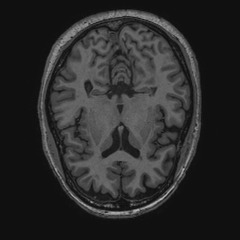
\includegraphics[width=.99\linewidth]{./images/t1.png}
 \end{minipage}
  \begin{minipage}{.24\textwidth}
 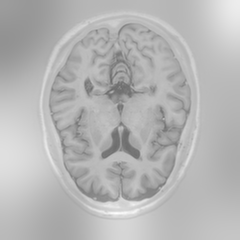
\includegraphics[width=.99\linewidth]{./images/t1-ir.png}
  \end{minipage}
  \begin{minipage}{.24\textwidth}
 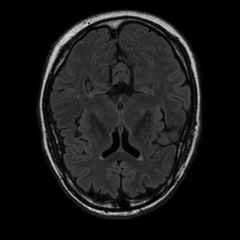
\includegraphics[width=.99\linewidth]{./images/t2-flair.png}
  \end{minipage}
  
   \begin{minipage}{.24\textwidth}
 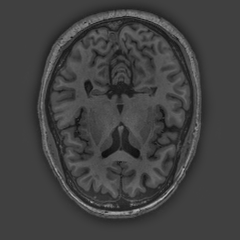
\includegraphics[width=.99\linewidth]{./images/t1-gs.png}
 \end{minipage}
  \begin{minipage}{.24\textwidth}
 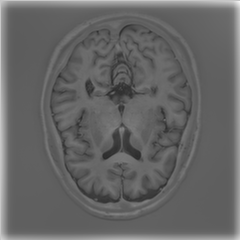
\includegraphics[width=.99\linewidth]{./images/t1-ir-gs.png}
  \end{minipage}
  \begin{minipage}{.24\textwidth}
 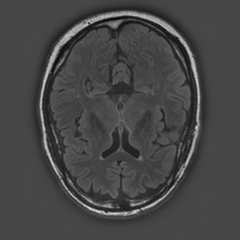
\includegraphics[width=.99\linewidth]{./images/t2-flair-gs.png}
  \end{minipage}
  \caption{Slice 19 of the 5th training sample. \emph{Top row (left to right):} T1, T1\_IR and T2\_FLAIR. \emph{Bottom row:} respective highpass filtered versions.}
  \label{data}
\end{figure}
We used the publicly available MrBrainS~\cite{mendrik2015mrbrains} challenge dataset, which was one of the datasets used to evaluate the PyraMiD-LSTM. The MrBrainS challenge data consists of 5 labeled samples and 15 testing samples, where each sample has a T1 weighted, T1 inversion recovery and a FLAIR scan. The additional high-resolution T1 scan was not used, as the labeling was performed on the low resolution data. The training data contained two different label maps, one for training and one for testing. The training map consists of classes for cortical gray matter (GM), basal ganglia, white matter (WM), WM lesions, cerebrospinal fluid (CSF), ventricles, cerebellum, brainstem and background. The testing map only defines classes for GM, WM and CSF, the respective classes of the training map are merged. Brainstem and cerebellum are not included in the evaluation and do therefore not appear labeled in the testing map.


\subsection{Convolutional Gated Recurrent Unit}\label{reordering}


The standard GRU as proposed in~\cite{cho_learning_2014} is defined as
\begin{align}
 r^j &= \sigma([W_r x]^j + [U_r h_{t-1}]^j),\\
 z^j &= \sigma([W_z x]^j + [U_z h_{t-1}]^j),\\
 \tilde{h}^j_t &= \phi([Wx]^j + [U(r \odot h_{t-1})]^j),\\
 h^j_{t} &= z^j\odot h^j_{t-1} + (1-z^j)\odot \tilde{h}^j_{t},
\end{align}
where $x$ is the input data, $r^j$ is the reset gate, $z^j$ is the update gate of the hidden unit $j$ and the activation is performed in $h^j$. The operator $\odot$ represents an elementwise multiplication. The functions $\sigma(\cdot)$ and $\phi(\cdot)$ stand for the logistic function and the hyperbolic tangent. $W$ and $U$ are the weight matrices for the current input and last step's output data respectively. Along the lines of Stollenga et al.~\cite{stollenga_parallel_2015}, we adapt these equations to be able to process 3D volumes and introduce our convolutional GRU (C-GRU):
\begin{align}\label{eq:cgru1}
 r^j &= \sigma \left( \sum\limits_i^I (x^i*w_r^{i,j}) + \sum\limits_k^J ( h_{t-1}^k*u_r^{k,j} ) +b^j_r\right),\\\label{eq:cgru2}
 z^j &= \sigma \left( \sum\limits_i^I (x^i*w_z^{i,j}) + \sum\limits_k^J ( h_{t-1}^k*u_z^{k,j} ) +b^j_z\right),\\\label{eq:cgru3}
 \tilde{h}^j_t &= \phi \left( \sum\limits_i^I (x^i*w^{i,j}) + r^j \odot \sum\limits_k^J ( h_{t-1}^k * u^{k,j} ) +b^j\right),\\
  h^j_{t} &= z^j\odot h^j_{t-1} + (1-z^j)\odot\tilde{h}^j_{t},
\end{align}
where $*$ represents a convolution. Compared to the vanilla GRU, we introduced slight changes. We decided to use a bias $b$ on each gate. We factored $r^j$ out of the convolution operation between $u$ and $h_{t-1}$. This change was motivated by the fact that an additional convolution would require $r$ to have twice the support it needs now because of the chained convolution. Moreover, we reorder the data for each C-RNN such that the two spatial dimensions are closest to memory, and the temporal dimension is ordered according to the temporal direction, as explained in the next paragraph. We motivated that decision with faster possible processing speeds on the GPU, since all convolutions now require data that lies close in memory. The computations of one C-GRU are visualized as a computational graph in Fig.~\ref{fig:network}a.

The MD-GRU consists of two times $D$ C-GRUs, where $D$ is the dimensionality of the image data and we need one C-GRU for each of the two directions. We set the input data of channel $i$ as $x^i \in \mathbb{R}^{S_1\times \cdots\times S_D}$. For each spatial dimension $d$, we create the copies $x^{i,d,-1}, x^{i,d,+1} \in \mathbb{R}^{S_d\times S_1\times \cdots\times S_D}$ of $x$ and apply the following data transformations:
\begin{align}
 x^{i,d,+1}(s_d, s_1, \dots, s_{D}) &= x^i(s_1, \dots, s_d,\dots, s_{D}),\\
 x^{i,d,-1}(S_d-s_d, s_1, \dots, s_{D}) &= x^i(s_1,\dots , s_d,\dots, s_{D}),
\end{align}
where $s_d$ is the index of the assigned dimension of the C-GRU and $S_d$ is the size of dimension $d$. The inverse operation is applied to $h^{j,d,+1},h^{j,d,-1} \in \mathbb{R}^{S_d\times S_1\times \cdots\times S_D}$ to gather the final output $h^j$:
\begin{align}
h^j(s_1,\dots, s_{D}) &= \sum\limits_{d=1}^D \left ( h^{j,d,+1}(s_d, s_1, \dots, s_{D}) + h^{j,d,-1}(S_d-s_d, s_1, \dots, s_{D}) \right ).
\end{align}

Figure~\ref{fig:network}b details this process for the MD-GRU. We apply the same technique for our implementation of the MD-LSTM.
\subsection{Experiments}
\subsubsection{Network}
We model our network similar to~\cite{stollenga_parallel_2015}. We include three multi-dimensional RNN (MD-RNN) layers of 16, 32 and 64 channels which are connected with pixelwise fully connected hidden layers of 25 and 45 channels respectively, each followed by a hyperbolic tangent activation function. The last MD-RNN is attached to a pixelwise fully connected layer with $c$ channels, the same number as classes in the data. We estimate the probabilities for each class using a softmax in the last layer and consequently choose the multinomial logistic loss for the training of our network. Figure~\ref{fig:network}c shows our network setup for the case of MD-GRU.


\begin{figure}
 \centering
 \subfloat[][C-GRU]{
          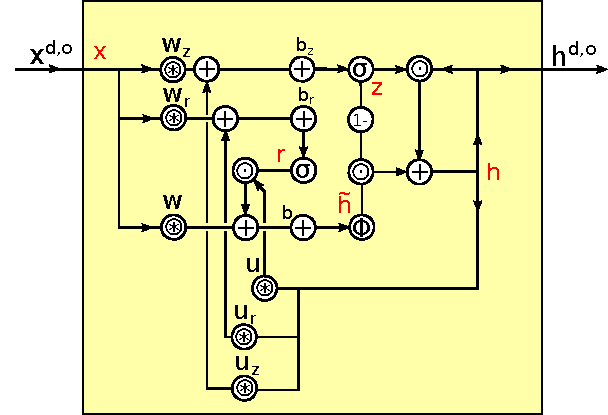
\includegraphics[width=0.35\textwidth]{images/cgrunotitle3.pdf}
 }\qquad
 \subfloat[][MD-GRU]{
          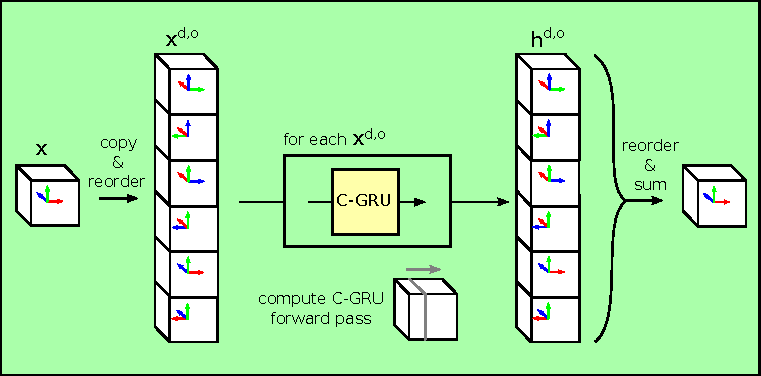
\includegraphics[width=0.48\textwidth]{images/mdgrunotitle2.pdf}
 }\quad
 
  \subfloat[][Network Architecture]{
          
\includegraphics[width=0.99\textwidth]{images/network.pdf}
 }
 \caption{(a) Directed graph denoting the computations in one C-GRU. The variables $x^{d,o}$, $h^{d,o}$ with $o \in \{-1,+1\}$ represent the input and output data across all $I$ and $J$ channels respectively. The $\circledast$ operator denotes here the sum per channel $j$ over the convolutions with each channel $i$ or $k$, as used in equations (\ref{eq:cgru1})--(\ref{eq:cgru3}). (b) Proposed arrangement of 6 C-GRUs in a MD-GRU for three-dimensional data. (c) Setup of our network.} \label{fig:network}
\end{figure}


\subsubsection{Setting}\label{setting}
All experiments were calculated on an NVIDIA GTX Titan X GPU with 12 GB global memory. Our implementation of MD-LSTM and MD-GRU relied on the fast convolution routines provided by NVIDIA's cuDNN~\cite{chetlur_cudnn:_2014}. For other layers, the already available implementations of the CAFFE\footnote{version 1.0.0-rc3, commit 9c46289} framework~\cite{jia2014caffe} were used.

\subsubsection{Preprocessing}
For all volumes, unsharp masking was done using a Gaussian smoothed image ($\sigma=5$~voxels) which was then subtracted from the original images to produce highpass filtered volumes. The original images and the highpass filtered images were normalized to $\sigma=1$ and $\mu=0$, assuming normally distributed values. In this way we followed a procedure similar to~\cite{stollenga_parallel_2015}, but omitted the histogram equalization. Figure \ref{data} shows the original and preprocessed data for training sample 5 at slice 19.

\subsubsection{Data augmentation}
In the training stage, at each iteration, a random location in the training data was selected and a deformation field was generated and applied to the subvolumes, which were then fed into the network. We used a procedure similar to~\cite{ronneberger_u-net:_2015}, but made the grid size dependent on the data. We did not use random deformations in the feasibility study mentioned in Sec.~\ref{feasibilitystudylabel}. For the testing phase, no deformations were applied.

\subsubsection{Training}
In three training steps we iteratively increase the subvolume size from $64\times64\times8$~voxels to $128\times128\times12$ and finally to $200\times200\times15$, keeping the third dimension smaller to account for the anisotropic MR volume resolution. We relied on AdaDelta~\cite{zeiler_adadelta_2012} to omit the manual tuning of a learning rate. For the challenge, we additionally used DropConnect~\cite{icml2013_wan13} of 0.5 on the input connections of each C-GRU to prevent overfitting. Training took around two days.


\subsubsection{Testing}
In the testing phase, we divided the volume into a grid of equally sized subvolumes of $120\times120\times8$, which were padded by 50, 50 and 4 voxels respectively on all sides of the volume. The padding was later used to stitch the results together using a Gaussian ($\mu=0$, $\sigma=(10,10,0.8)$) to produce interpolation weights, since the borders contain starting artifacts from the individual RNNs and do not contain adequate results. Since we trained for nine classes, but only four classes were needed for the final evaluation, we simply combined the binary labels for the CSF with the ventricles, the cortical GM with the basal ganglia and the WM with the WM lesions. Everything else was considered background. Testing one volume of the MRBrainS data required 32 iterations, which needed around two minutes.


\section{Results}

\subsection{Feasibility Study}
\label{feasibilitystudylabel}
\begin{table}
\caption{Feasibility study. Dice coefficients in percent for gray and white matter (GM/WM), cerebrospinal fluid (CSF) and intracranial volume (ICV).}% The case with more memory was only trained until iteration 28000}
\begin{center}
\begin{tabular}{lllll}\toprule
× & GM & WM & CSF & ICV\\ \midrule
MD-LSTM  & \textbf{88.09}  & 90.08 & 82.62  & 97.56 \\ 
MD-GRU & 87.88 & \textbf{90.15 } & \textbf{83.19} & \textbf{97.73 }\\ \bottomrule
\end{tabular}
\label{feasibilityquantitative}
\end{center}
\end{table}

\begin{figure}
 \centering
 \begin{minipage}{.24\textwidth}
 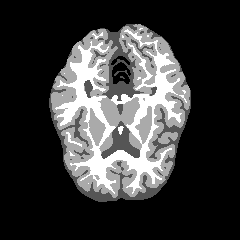
\includegraphics[width=.98\linewidth]{./images/lstmfeas_new_new.png}
 \end{minipage}
  \begin{minipage}{.24\textwidth}
 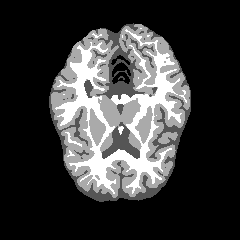
\includegraphics[width=.98\linewidth]{./images/grusfeas_new_new.png}
  \end{minipage}
  \begin{minipage}{.24\textwidth}
 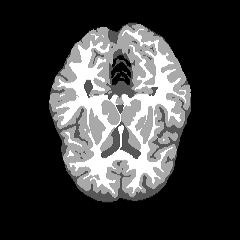
\includegraphics[width=.98\linewidth]{./images/Traindata5atslice19-Testlabel.png}
  \end{minipage}
  
  \begin{minipage}{0.80\textwidth}
    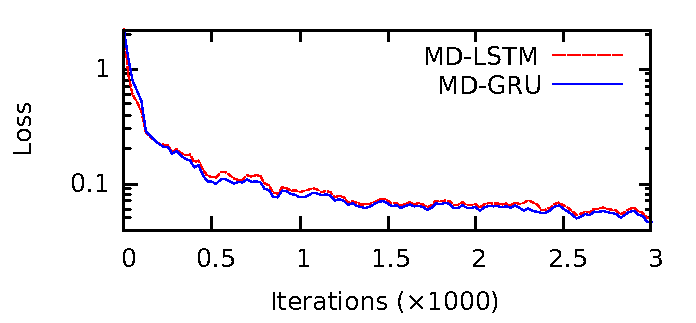
\includegraphics[width=.9\linewidth]{./images/convergence_rate_new10000_mediumlines_withtitle6.pdf}
  \end{minipage}
  \caption{Feasibility study. \emph{Top row:} slice 19 of the 5th training volume used for the evaluation. The images from left to right represent the results of the MD-LSTM, the MD-GRU and the manual labeling. \emph{Bottom row:} convergence rates for the feasibility study of both MD-GRU and MD-LSTM.}
\label{feasibilityqualitative}

\end{figure}
To point out differences between the MD-GRU and the MD-LSTM, we ran the same setup with the multi-dimensional RNN layers either being an MD-GRU or an MD-LSTM. We used the first four volumes in the training set of the MrBrainS challenge and trained both networks for 3\,000 iterations on the largest possible resolution which was feasible for both (limited to $192\times192\times14$ by our MD-LSTM implementation). On average, one training iteration for MD-GRU and MD-LSTM took 9.1 and 12.8 seconds, respectively. The Dice coefficients for CSF, GM, WM and ICV between the computed segmentation of the 5th training volume and the provided reference segmentation are shown in Table~\ref{feasibilityquantitative} for both the MD-GRU and MD-LSTM. Slice 19 of the computed segmentations and the reference segmentation are displayed in Fig.~\ref{feasibilityqualitative} together with a plot of a running average of 100 iterations of the loss function for each iteration of the training procedure.


\subsection{MD-GRU on MRBrainS}
In our attempt to beat the highscore of the MRBrainS challenge, we used our described data augmentation method. Each subvolume was deformed randomly throughout all three training phases. We used all provided low resolution volumes and their highpass filtered versions. Table~\ref{mrbrainsres} lists our performance according to the Dice coefficients, 95th-percentile  of the Hausdorff distance and average volume difference of the GM, WM, CSF and ICV. Nine measures were relevant for the final evaluation: Dice, modified Hausdorff distance and average volume distance in each of the categories GM, WM and CSF. The sum of the ranks in these nine categories is used as the performance score and determines the final rank. 
Figure~\ref{visualresultschallenge} shows the computed segmentation at slice 19 of samples 5, 10 and 15 of the test data. 
\begin{table}
\begin{center}
 \caption{MrBrainS challenge. Results of the six best performing methods for GM, WM, CSF and ICV of all three used metrics (Dice, 95th-percentile of the Hausdorff distance (HD) and average volume difference (AVD)). A bold number means best out of these six. The results reflect the state on August 12, 2016.}
\label{mrbrainsres}
 \scriptsize
\begin{tabular}{l c rcl rcl rcl rcl rcl}
\toprule
Team name &  Rank &\multicolumn{3}{c}{GM} & \multicolumn{3}{c}{WM} & \multicolumn{3}{c}{CSF} &  \multicolumn{3}{c}{ICV}\\%\hline\hline
×& × & Dice & HD & AVD & Dice & HD & AVD & Dice & HD & AVD & Dice & HD & AVD \\\midrule
CU\_DL2  & \textbf{1}& \textbf{86.15} & \textbf{1.45} & 6.60 & \textbf{89.46} & \textbf{1.94} & 6.05 & \textbf{84.25}& 2.19 & 7.69 &  98.10 & 2.75 & 1.54\\
CU\_DL& 2  & 86.12 & 1.47 & 6.42 & 89.39 & \textbf{1.94} & \textbf{5.84} & 83.96 & 2.28 & 7.44 &  97.99 & 3.16 & 1.83 \\
MD-GRU [proposed] & 3 & 85.40 & 1.55 & \textbf{6.09} & 88.98 & 2.02 & 7.69 & 84.13 & 2.17 & 7.44 & \textbf{98.15} & \textbf{2.37} & 0.86\\
PyraMiD-LSTM2 & 4 & 84.89 & 1.67 & 6.35 & 88.53 & 2.07 & 5.93 & 83.05 & 2.30 & 7.17 &  98.04 & 2.86 & \textbf{0.69}\\
FBI/LMB Freiburg~\cite{cicek_3d_2016}& 5 & 85.44 & 1.58 & 6.60 & 88.86 & 1.95 & 6.47 & 83.47 & 2.22 & 8.63 &  97.98 & 2.51 & 1.06\\
IDSIA~\cite{stollenga_parallel_2015} & 6 & 84.82 & 1.70 & 6.77 & 88.33 & 2.08 & 7.05& 83.72 & \textbf{2.14} & \textbf{7.09}& \textbf{98.15} & 2.44 & 0.95\\\bottomrule
\end{tabular}
\end{center}
 \label{resultschallenge}
\end{table}

\begin{figure}
 \centering
 \begin{minipage}{.24\textwidth}
 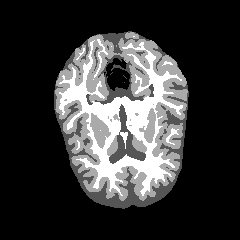
\includegraphics[width=.99\linewidth]{./images/sl19-v5-test-challres_new.png}
 \end{minipage}
  \begin{minipage}{.24\textwidth}
 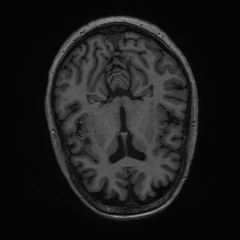
\includegraphics[width=.99\linewidth]{./images/sl19-v5-test-t1.png}
  \end{minipage}
  \begin{minipage}{.24\textwidth}
 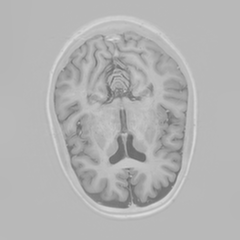
\includegraphics[width=.99\linewidth]{./images/sl19-v5-test-t1-ir.png}
  \end{minipage}
  \begin{minipage}{.24\textwidth}
 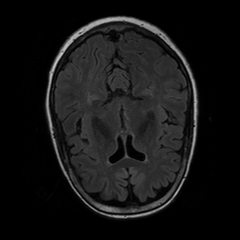
\includegraphics[width=.99\linewidth]{./images/sl19-v5-test-t2-flair.png}
  \end{minipage}
  
  \vspace{0.3em}
   \begin{minipage}{.24\textwidth}
 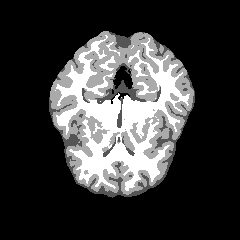
\includegraphics[width=.99\linewidth]{./images/sl19-v10-test-challres_new.png}
 \end{minipage}
  \begin{minipage}{.24\textwidth}
 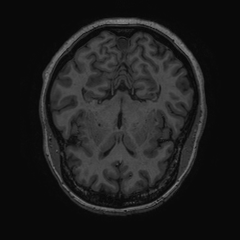
\includegraphics[width=.99\linewidth]{./images/sl19-v10-test-t1.png}
  \end{minipage}
  \begin{minipage}{.24\textwidth}
 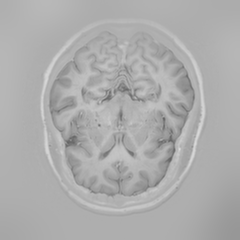
\includegraphics[width=.99\linewidth]{./images/sl19-v10-test-t1-ir.png}
  \end{minipage}
  \begin{minipage}{.24\textwidth}
 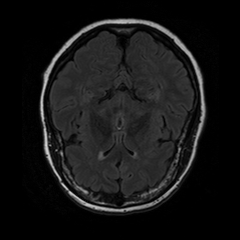
\includegraphics[width=.99\linewidth]{./images/sl19-v10-test-t2-flair.png}
  \end{minipage}
  
  \vspace{0.3em}
   \begin{minipage}{.24\textwidth}
 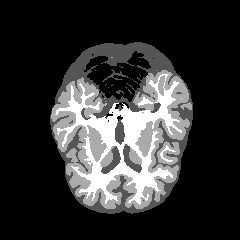
\includegraphics[width=.99\linewidth]{./images/sl19-v15-test-challres_new.png}
 \end{minipage}
  \begin{minipage}{.24\textwidth}
 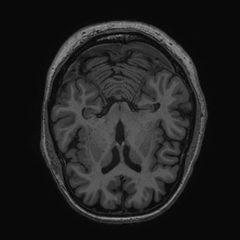
\includegraphics[width=.99\linewidth]{./images/sl19-v15-test-t1.png}
  \end{minipage}
  \begin{minipage}{.24\textwidth}
 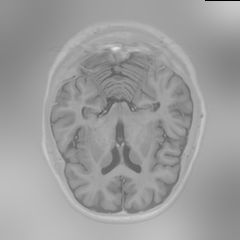
\includegraphics[width=.99\linewidth]{./images/sl19-v15-test-t1-ir.png}
  \end{minipage}
  \begin{minipage}{.24\textwidth}
 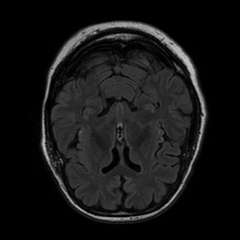
\includegraphics[width=.99\linewidth]{./images/sl19-v15-test-t2-flair.png}
  \end{minipage}
  \caption{MrBrainS challenge. \emph{Rows (top to bottom):} 5th, 10th and 15th test sample. \emph{Columns (left to right):} slice 19 of our segmentation results, T1, T1\_IR and T2\_FLAIR.}
   \label{visualresultschallenge}

\end{figure}



\section{Discussion}

The feasibility study has shown that MD-GRU has great potential for the segmentation of volumetric images, since it achieved comparable results to the MD-LSTM in less time with the same settings. 

Using deformation as a data augmentation strategy and DropConnect for regularization in the challenge, we ranked 3rd out of 37. Unfortunately, none of the results in the top five of the challenge highscore are published so far. The 4th and 6th entries are both incarnations of the already discussed MD-LSTM, where only the latter was described in~\cite{stollenga_parallel_2015} and the former likely contains unpublished improvements to their method. In contrast to \cite{stollenga_parallel_2015}, we did not omit the original T1\_IR images. Yet some obvious misclassifications could be traced back to strong bias field artifacts in the T1\_IR images. Given the small training size, using the T1\_IR images leads to apparent fitting to the bias field. Furthermore, we were not able to replicate the training volume size of Stollenga et al.~\cite{stollenga_parallel_2015} due to a higher memory requirement of our implementation, since we decided to copy the input and output data for each RNN layer, as detailed in Sec.~\ref{reordering}. This has to be kept in mind when comparing the two approaches. Relationships between areas that are located at a certain distance in the data could therefore not be modeled in our network, where~\cite{stollenga_parallel_2015} was able to use the full spatial context in two dimensions as well as a larger third dimension. In their last training step more than half of the data was covered while we could only fit a bit more than a fifth in our memory. 

The contribution on rank five was computed using the 3D U-Net~\cite{cicek_3d_2016}. It consists of a hierarchical convolutional neural network with shortcut connections, which is trained using various on-the-fly data augmentation techniques, including the deformation strategy used in this paper. The challenge results and corresponding adaptations of the algorithm to fit the challenge data are, however, not yet published. We believe that data augmentation is key for successful applications to problems with such a small training size. 


 \subsubsection{Conclusion}
 With the MD-GRU, we combined the enormous expressive power of RNNs with a highly beneficial data augmentation strategy, resulting in a powerful supervised automatic segmentation technique. With a memory-savvy implementation that omits the initial reordering of the data, results surpassing the state of the art should be possible with MD-GRU.



\bibliographystyle{splncs03}
\bibliography{manuallib}
\end{document}
